\documentclass{article}
\usepackage[final]{listings}
\usepackage{color}
\usepackage{float}
\usepackage{xcolor}

\usepackage{caption}
\DeclareCaptionFont{white}{\color{white}}
\DeclareCaptionFormat{listing}{\colorbox{gray}{\parbox{\textwidth}{#1#2#3}}}
\captionsetup[lstlisting]{format=listing,labelfont=white,textfont=white}

\usepackage{graphicx}
\usepackage{enumerate}
\usepackage[latin1]{inputenc} 
\usepackage[spanish]{babel}
\lstset{language=Octave}

\begin{document}
\begin{center}
\textbf{
{\LARGE Promen 2, Problema 3\\
Embalse retardador de crecidas\\
M\'etodos Num\'ericos\\
ITBA\\
}}
\end{center}
\vspace{8cm}

Primer autor:\\
\textbf{Conrado Mader Blanco} - Legajo 51270 (Comisi\'on S, lunes)\\
\textit{cmaderbl@alu.itba.edu.ar}\\

Co-autores:\\
\textbf{Betina Cynthia Mamani} - Legajo 52310 (Comisi\'on B, lunes)\\
\textbf{Federico Ramundo} - Legajo 51596 (Comisi\'on S, lunes)\\
\newpage

\section{Enunciado completo del problema}
\subsection{Determinaci\'on del problema}

La determinaci\'on del problema se realiza de acuerdo a las pautas determinadas por la c\'atedra. Para ello, se ejecuta el comando: octave nro\_prob.m\\

El mismo determina que el problema a realizar es el n\'umero 3.\\
\subsection {Enunciado}

Suponga un embalse que supondremos tiene como principal prop\'osito actuar como retardador de crecidas en un curso de agua. Al ingresar agua al embalse por alg\'un afluente o una tormenta, el nivel de agua en el mismo asciende y si se excede cierta cota H entonces se produce un caudal de salida desde el embalse hacia aguas abajo. Se conoce el flujo de entrada al embalse en funci\'on de tiempo (lo denominaremos hidrograma de entrada $E(t))$. Para el hidrograma de salida $S(t)$ (flujo de salida del embalse hacia aguas abajo) se tiene una estructura (el vertedero) en la que $S(t)$ depende de la diferencias de alturas $h ? H$, donde ambas alturas se miden desde el punto mas profundo del embalse siendo h la distancia entre la superficie libre y ese punto de mayor profundidad. Del embalse se conoce el \'area $A(z)$ de cada secci\'on horizontal del mismo como funci\'on de la distancia z al punto mas profundo.
Se puede plantear un modelo elemental de flujos de entrada y salida para obtener el siguiente problema de valor inicial del cual es soluci\'on $h(t)$:\\
\begin{displaymath}
h(t) =\frac{(E(t) - S(t))}{A(h(t))}
\end{displaymath}
\begin{displaymath}
 t \in [0, T ],	h(0) = h0
\end{displaymath}
De las funciones $A(h)$ y $E(t)$ se dispondr\'a solo la informaci\'on de una tabla de valores en las que se podr\'a interpolar en el caso que hiciesen falta valores no registrados. Se supondr\'a
que 
\begin{displaymath}
S(t) = \left\{
\begin{array}{cl}
C \sqrt{(h(t) -H)^3}&\mbox{si } h(t)>H\\
0&\mbox{si } h(t)<H
\end{array}\right.
\end{displaymath}
 con $C$ una constante positiva.\\
 
 \begin{enumerate}
\item Se desea analizar el comportamiento del embalse como atenuador del pico de crecida y como retardador de la aparici\'on de dicho pico. Supondremos conocido el flujo de entrada $E(t)$ con $t$ en miles de segundos y $E$ en $m^3/s$ como indica la siguiente tabla:\\\\
 \begin{tabular}{|c|c|c|c|c|c|c|c|c|c|c|c|}
\hline
$t$& 0.0 &  1.8 & 3.6 & 5.4 & 7.2 & 9.0 & 10.8 & 12.6 & 14.4 & 16.2 & 18.0\\ \hline
E &  0 & 30 & 150 & 400 & 500 & 460 & 350 & 230 & 130 & 60 & 10\\ \hline
\end{tabular}\\
\\De la funci\'on $A(h)$ se conoce la siguiente tabla de valores con $h$ en metros y $A$ en miles de $m^2$:\\\\
\begin{tabular}{|c|c|c|c|c|c|c|c|c|c|c|}
\hline
$h$ & 0.0 &  2.5 & 5.0 & 7.5 & 10.0 & 12.5 & 15.0 & 17.5 & 20.0 & 22.5 \\ \hline
$A$ &  0.0 & 0.1 & 1.4 & 7.0 & 18.5 & 42.0 & 80.0 & 140.0 & 230.0 & 330.0 \\ \hline
\end{tabular}\\\\
\begin{tabular}{|c|c|c|c|c|c|}
\hline
$h$& 25.0 & 27.5 & 30.0 & 32.5 & 35.0 \\ \hline
$A$& 480.0 & 700.0 & 1000.0 & 1100.0 & 1600.0 \\ \hline
\end{tabular}\\
\\Obtener $h(t)$ integrando el problema de valor inicial con el m\'etodo de Runge-Kutta de orden 4 suponiendo un paso de 100 segundos con $T = 30000$ segundos si $H = 30$ metros, $C=30$(en el MKS) y $h0 =H$. Para evaluar las funciones $E$ y $A$ se sugiere usar el procedimiento $interp1$ en Octave para implementar una interpolaci\'on por splines. Para $t$ mayor que 18000 segundos suponga que $E(t)$ es cero.\\
 
\item Representar gr\'aficamente $h(t)$ identificando su valor m\'aximo y el instante en que se produce.\\
\item En un mismo gr\'afico representar $E(t)$ y $S(t)$ y comentar el efecto que produce el embalse atenuando y retardando el fen\'omeno de crecida. Con los resultados obtenidos estimar la raz\'on $R$ entre los picos de $E$ y $S$ as\'i como el retardo $D$ entre la aparici\'on de ambos picos.\\
 
\item Completar una tabla con los valores de $R$ y $D$ si los datos de entrada de $E$ se multiplican por: 0.5, 0.75, 1 (que fueron obtenidos),1.25 y 1.5.\\
 \end{enumerate}
 \newpage
 \section{Planteo del problema y resultados obtenidos}
 
 \subsection{item 1}
 
Utilizando el m\'etodo de Runge-Kutta de orden 4 obtuvimos una aproximaci\'on a $h(t)$ cuyos valores no mostramos a continuaci'on dado que al aproximar de $t = 0$ a $30000$ con un salto de $100$ obtuvimos una tabla de 301 entradas, lo cual resulta muy extenso. El gr\'afico pertinente a $h(t)$ puede verse en el siguiente item.
 
 \subsection{item 2}
El gr\'afico de la aproximaci\'on de $h(t)$ puede verse en la figura \ref{fig:item2}.\\
\begin{figure}[H]
\centering
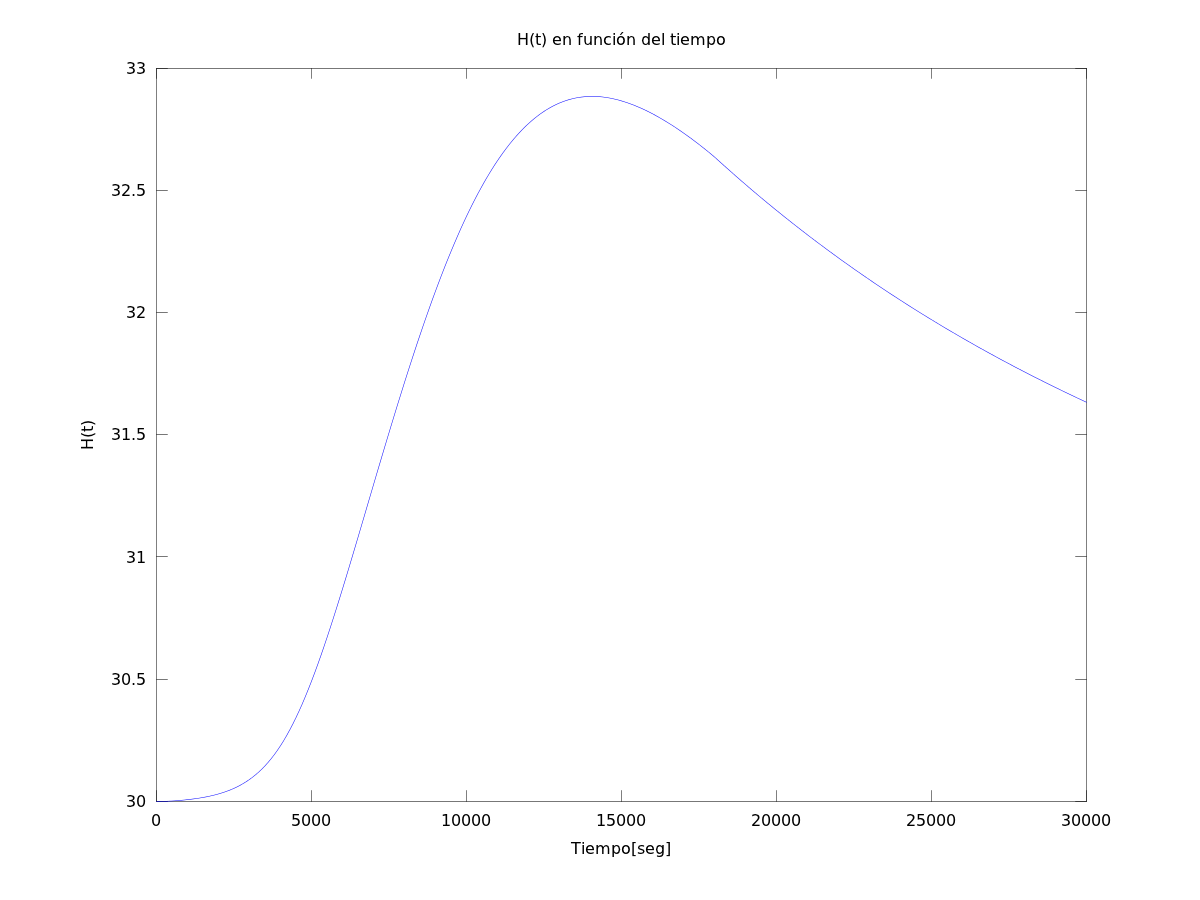
\includegraphics[scale=0.3]{../graficos/grafico_item2.png}
\caption{ Gr\'afico de la aproximaci\'on de $h(t)$ en funci\'on del tiempo.}
\label{fig:item2}
\end{figure}
Los resultados que obtuvimos respecto al m\'aximo de $h(t)$ y al tiempo en el que ocurre son:\\
\begin{displaymath}
 \begin{array}{cc}
$m\'aximo $ =  32.884 m\\
$instante $ = 14100 seg
\end{array}
 \end{displaymath}

\subsection{item 3}
 
En la figura \ref{fig:item3} pueden observarse graficadas las funciones $E(t)$ y $S(t)$.\\
\begin{figure}[H]
\centering
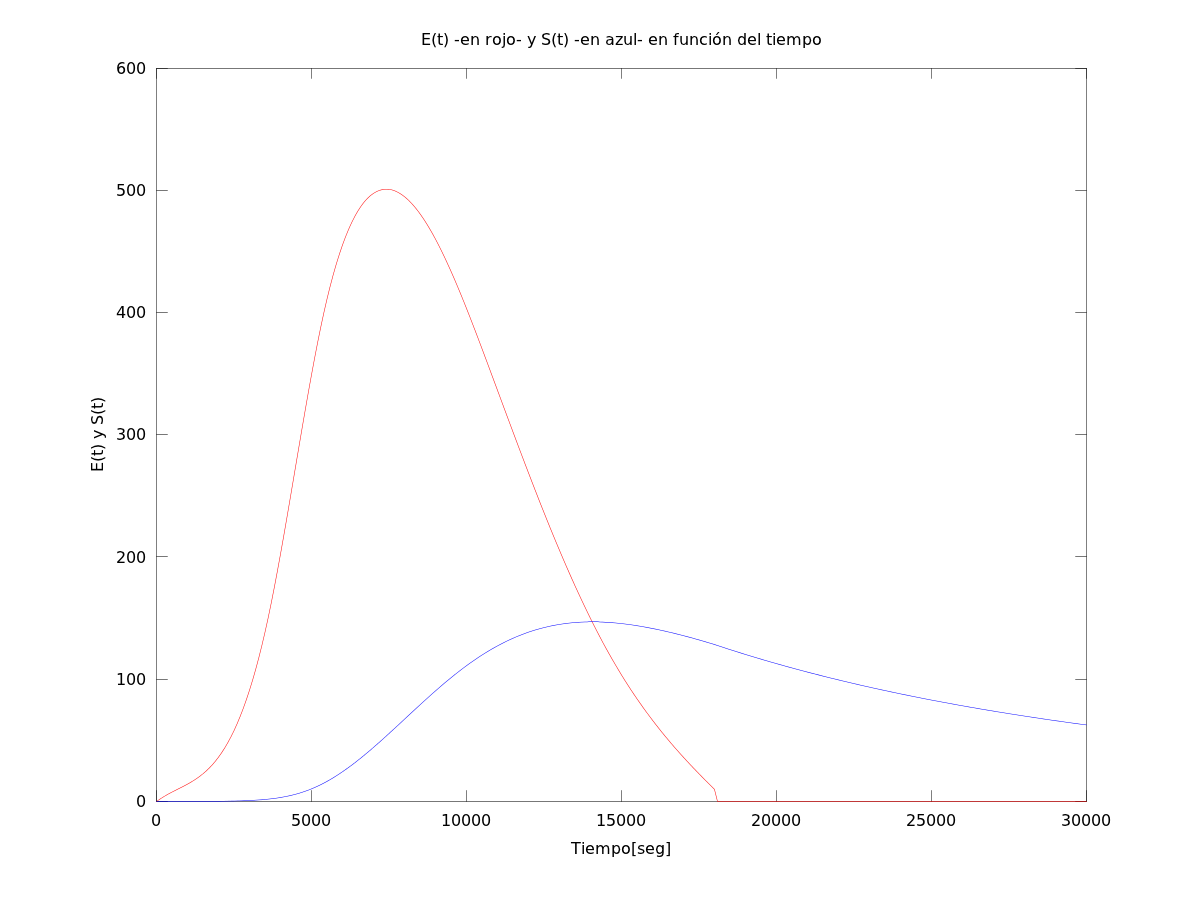
\includegraphics[scale=0.3]{../graficos/grafico_item3.png}
\caption{ Gr\'afico de $E(t)$ y $S(t)$ en funci\'on del tiempo.}
\label{fig:item3}
\end{figure}
El efecto que produce el embalse atenuando y retardando el fen\'meno de crecida, como se observa en el gr\'afico, es una fuerte subida en la entrada del embalse ($E(t)$) seguida de una fuerte ca\'da, mientras que la salida ($S(t)$) no describe un pico tan pronunciado y lo alcanza con cierto retarde respecto de la entrada (dado que para que salga agua del embalse primero debe entrar). \\
Mientras que el m\'aximo de la salida no es tan elevado como el de la entrada, su crecimiento y su decrecimiento son m\'as suaves si se comparan con los de la entrada  ($E(t)$).\\
Cabe destacar que tanto en al entrada como en al salida, una vez alcanzado el pico, la pendiente de decrecimiento es menos pronunciada que en la de crecimiento.\\
La raz\'on $R$ entre los picos de $E$ y $S$, y el retardo $D$ entre ambos picos, seg\'un los c\'alculos obtenidos es el siguiente:
 \begin{displaymath}
 \begin{array}{cc}
R =  3.4088\\
D =  6700 seg
\end{array}
 \end{displaymath}
 
 \subsection{item 4}
Multiplicando $E(t)$ por los siguientes factores, los resultados que obtuvimos de la relaci\'on $R$ entre los picos de $E(t)$ y $S(t)$ y la distancia $D$ corresponden a la siguiente tabla:\\
\begin{center}
 \begin{tabular}{|c|c|c|}
 \hline
 Factor & $R$ & $D [seg]$ \\\hline
   0.50 &   1.7044 & 6700 \\\hline
   0.75 &   2.5566 & 6700 \\\hline
   1.00 &   3.4088 & 6700 \\\hline
   1.25 &   4.2610 & 6700 \\\hline
   1.50 &   5.1133 & 6700 \\\hline

 \end{tabular}
 \end{center}
Resulta interesante el hecho de que por mas que cambiemos los valores de $E(t)$ el retardo entre los picos de \'esta y $S(t)$ se mantiene constante, dado que multiplicarla por un escalar tan solo hace que var\'e su valor num\'erico, pero no afecta al instante en que alcanza su m\'aximo .
 \newpage
 \section{C\'odigos Octave}
 \begin{lstlisting}[frame=tblr,breaklines=true]
function ret = nro_prob( legajos )

%
% Determina el n\'umero de problema a 
% realizar por el grupo
%

    ret = rem( min(legajos), 4 ) + 1;

end

disp( nro_prob( [ 51270 52310 51596 ] ) );

\end{lstlisting}
\begin{itemize}
\item \'Item 1
\begin{lstlisting}[frame=tblr,breaklines=true]

%
% Interpola por spline utilizando el m�todo
%  interp1 sugerido
%

function y = interpolar(X, Y, x)

    [y] = interp1(X, Y, [x], 'spline');

end

%
% Evalua la funci�n E de entrada de agua 
% al embalse
%

function y = E(t, factor)

    if(t > 18000)
        y = 0;

    else
        y = interpolar([0: 1800: 18001], [0, 30, 150, 400, 500, 460, 350, 230, 130, 60, 10] .* factor, t);
    end

end

%
% Evalua la funci�n A de secci�n horizontal 
% del embalse
%

function y = A(t)

    a = [0: 2.5: 35];
    b = [0, 100, 1400, 7000, 18500, 42000, 80000, 140000, 230000, 330000, 480000, 700000, 1000000, 1100000, 1600000];

    y = interpolar(a, b, t);

end

%
% Evalua la funci�n S de salida de agua del embalse
%

function y = S(h, h0, C)

    if(h <= h0)
        y = 0;

    else
        y = C * (h - h0) ^ (3/2);
    end

end

%
% Funci�n f(t_k, y_k) utilizada por el m�todo de 
% Runge-Kutta para aproximar h(t). 
% Equivale a la funci�n h'(t) del enunciado.
%

function y = f(tk, yk, h0, C, factor)

    y = (E(tk, factor) - S(yk, h0, C)) / A(yk);

end

%
% Ejecuta el m�todo de Runge-Kutta
% de orden 4
%

function Y = runge_kutta4(ti, tf, step, h0, C, factor)

    Y = [h0];

    for t = ti:step:(tf - step)

        yk = Y(length(Y));

        k1 = step * f(t, yk, h0, C, factor);
        k2 = step * f(t + step/2, yk + k1/2, h0, C, factor);
        k3 = step * f(t + step/2, yk + k2/2, h0, C, factor);
        k4 = step * f(t + step, yk + k3, h0, C, factor);

        Y = [Y, yk + (k1 + 2*k2 + 2*k3 + k4)/6];

    end

end
\end{lstlisting}
\item \'Item 2
\begin{lstlisting}[frame=tblr,breaklines=true]

%
% Grafica la funci�n h(t)
%

function graficar_item2(H, T, nombre)

    plot(T, H);
    title('H(t) en funci\'on del tiempo');
    xlabel('Tiempo[seg]');
    ylabel('H(t)');

    print(nombre, '-dpng');

end

%
% Calcula el maximo en h(t)
%

function [M, tM] = calcular_maximo(H, T)

    [M, tM] = max(H);

    tM = T(tM);

end

\end{lstlisting}
\item \'Item 3
\begin{lstlisting}[frame=tblr,breaklines=true]
source("item1.m");

%
% Calcula dos vectores
% equivalentes a E(t) y a S(t)
%

function [vectorE, vectorS] = calcular_vectores(H, T, C, factor)

    vectorS = [];

    for h=H

        vectorS = [vectorS, S(h, H(1), C)];

    end

    vectorE = [];

    for t=T

        vectorE = [vectorE, E(t, factor)];

    end

end

%
% Grafica E(t) y S(t)
%

function graficar_item3(H, T, C, nombre, factor)

    [vectorE, vectorS] = calcular_vectores(H, T, C, factor);

    plot(T, vectorE, 'r', T, vectorS, 'b');
    title('E(t) -en rojo- y S(t) -en azul- en funci\'on del tiempo');
    xlabel('Tiempo[seg]');
    ylabel('E(t) y S(t)');

    print(nombre, '-dpng');

end

%
% Calcula los picos y el retardo entre ellos
%

function [R, D] = calcular_picos(H, T, C, factor)

    [vectorE, vectorS] = calcular_vectores(H, T, C, factor);

    [maxE, posMaxE] = max(vectorE);
    [maxS, posMaxS] = max(vectorS);

    R = maxE / maxS;

    D = abs(T(posMaxE) - T(posMaxS));

end


\end{lstlisting}
\item \'Item 4
\begin{lstlisting}[frame=tblr,breaklines=true]
source("item3.m");

%
% Crea la tabla con los valores de R y D 
% multiplicando E por 0.5, 0.75, 1, 1.25 y 1.5
%

function tabla_item4(H, T, C)

    tabla = [];

    for factor = 0.5:0.25:1.5

        [R, D] = calcular_picos(H, T, C, factor);
        tabla = [tabla, transpose([factor, R, D])];

    end

    printf("\n\tFactor\tR\tD\n");

    transpose(tabla)

end

\end{lstlisting}
\end{itemize}
\newpage
\section{Conclusiones}

Podemos concluir que el m\'etodo de Runge-Kutta de orden 4 resulta muy \'util a la hora de aproximar una funci\'on, conociendo su derivada y un valor inicial. Permite aproximarse al valor real de la funci\'on con un error mucho menor que otros m\'etodos como el de Heun (orden 2) o el de Euler (orden 1), y el hecho de automatizar el proceso evita la parte engorrosa de calcular todos los t\'erminos intermedios K1, K2, K3 y K4 que se necesitan para pasar de un  $y_k$ a un $y_{k+1}$.\\

Adem\'as, consideramos de gran utilidad  la utilizaci\'on del Software Octave con el objetivo de resolver problemas f\'isico-matem\'aticos. El lenguaje utilizado por Octave no es tipado, lo que resulta muy c\'omodo a la hora de realizar c\'alculos y programar funciones, a lo que si a esto se le suma la potencia del GNU Plot, resulta realmente pr\'actico dado que es posible computar y graficar todos los resultados de los problemas planteados.\\

Por \'ultimo, cabe destacar que la precisi\'on con la que se obtuvo el resultado puede ser ajustado por el usuario, obviamente dentro de las limitaciones de la arquitectura del sistema en que se est\'a trabajando.\\

Este trabajo nos result\'o interesante como equipo dado que refleja el hecho de que los conocimientos adquiridos en la materia pueden ser aplicados perfectamente a problemas de la vida real, ayudando a minimizar costos, agilizar procesos, etc. 

\end{document}